\documentclass[aspectratio=169]{beamer}

\usetheme{UiO}

\usepackage{emoji}
\usepackage{pgfplots}

\usetikzlibrary{overlay-beamer-styles}

\title{Integrating complex multimodal health data for clinical prediction with artificial intelligence}
\author{Esten H. Leonardsen}
\date{\today}

\def\systemfont{\footnotesize}

\def\vsep{0.5}
\def\hsep{0.65}
\def\edgeopacity{0.5}

\newcommand{\neuron}[3][uiogreen]{
    \node[circle, draw=black, fill=#1, minimum size=0.3cm] (#2) at #3 {};
}
\newcommand{\nn}[2]{
    \begin{tikzpicture}
        \node[fill=gray!80, minimum width=3cm, minimum height=2cm, rounded corners=0.1cm, text=white, draw=black, font=\systemfont, anchor=south, text depth=1.5cm] (#2) at (0, 0) {
            #1
        };


        \neuron{n20}{($ (#2.south) + (0, 0.75) + (-1*\hsep, -1*\vsep) $)}
        \neuron{n21}{($ (n20) + (0, \vsep) $)}
        \neuron{n22}{($ (n20) + (0, 2*\vsep) $)}

        \neuron{n30}{($ (n20) + (\hsep, 0.5*\vsep) $)}
        \neuron{n31}{($ (n20) + (\hsep, 1.5*\vsep) $)}

        \neuron{n40}{($ (n20) + (2*\hsep, \vsep) $)}

        \foreach \j in {0,...,2} {
            \draw[black, opacity=\edgeopacity] ($ (#2.south west) + (0, 0.75) $) -- (n2\j);
        }

        \foreach \j in {0,...,2} {
            \foreach \k in {0,...,1} {
                \draw[black, opacity=\edgeopacity] (n2\j) -- (n3\k);
            }
        }
        \draw[black, opacity=\edgeopacity] (n30) -- (n40);
        \draw[black, opacity=\edgeopacity] (n31) -- (n40);
        \draw[black, opacity=\edgeopacity] (n40) -- ($ (#2.south east) + (0, 0.75) $);
    \end{tikzpicture}
}
\newcommand{\encoder}[2]{
    \begin{tikzpicture}
        \node[fill=gray!80, minimum width=2cm, minimum height=1.9cm, rounded corners=0.1cm, text=white, draw=black, font=\systemfont, anchor=south, text depth=1.4cm] (#2) at (0, 0) {
            #1
        };


        \neuron{#2n20}{($ (#2.south) + (0, 0.75) + (-0.5*\hsep, -1*\vsep) $)}
        \neuron{#2n21}{($ (#2n20) + (0, \vsep) $)}
        \neuron{#2n22}{($ (#2n20) + (0, 2*\vsep) $)}

        \neuron{#2n30}{($ (#2n20) + (\hsep, 0.5*\vsep) $)}
        \neuron{#2n31}{($ (#2n20) + (\hsep, 1.5*\vsep) $)}

        \foreach \j in {0,...,2} {
            \draw[black, opacity=\edgeopacity] ($ (#2.south west) + (0, 0.75) $) -- (#2n2\j);
        }

        \foreach \j in {0,...,2} {
            \foreach \k in {0,...,1} {
                \draw[black, opacity=\edgeopacity] (#2n2\j) -- (#2n3\k);
            }
        }
    \end{tikzpicture}
}


\begin{document}
	\begin{frame}
	 	\titlepage
	\end{frame}

	\newcommand{\mriside}[4]{
    \def\mridepth{0.75}

    \node[inner sep=0pt] (input) at (#1, #2) {
        \includegraphics[height=#3, width=#3]{#4}
    };

    \draw[fill=black] (input.north west) --
        ($ (input.north west) + (0.5 * \mridepth, 0.5 * \mridepth) $) --
        ($ (input.north east) + (0.5 * \mridepth, 0.5 * \mridepth) $) --
        (input.north east) -- cycle;
    \draw[fill=black] (input.north east) --
        ($ (input.north east) + (0.5 * \mridepth, 0.5 * \mridepth) $) --
        ($ (input.south east) + (0.5 * \mridepth, 0.5 * \mridepth) $) --
        (input.south east) -- cycle;
    \draw[] (input.north west) --
        ($ (input.north west) - (0.5 * \mridepth, 0.5 * \mridepth) $) --
        ($ (input.south west) - (0.5 * \mridepth, 0.5 * \mridepth) $) --
        (input.south west) -- cycle;
    \draw[] (input.north east) --
        ($ (input.north east) - (0.5 * \mridepth, 0.5 * \mridepth) $) --
        ($ (input.south east) - (0.5 * \mridepth, 0.5 * \mridepth) $) --
        (input.south east) -- cycle;
    \draw[] ($ (input.north west) - (0.5 * \mridepth, 0.5 * \mridepth) $) --
        ($ (input.north east) - (0.5 * \mridepth, 0.5 * \mridepth) $);
    \draw[] ($ (input.south west) - (0.5 * \mridepth, 0.5 * \mridepth) $) --
        ($ (input.south east) - (0.5 * \mridepth, 0.5 * \mridepth) $);
}


\newcommand{\inputside}[3]{
    \mriside{#1}{#2}{#3}{data/mri_sagittal.png}
}

\newcommand{\heatmapside}[3]{
    \mriside{#1}{#2}{#3}{data/combined_sagittal.png}
}

\newcommand{\convside}[6]{
    \def\sidex{#1}
    \def\sidey{#2}
    \def\sidewidth{#3}
    \def\sideheight{#4}
    \def\sidefillcolour{#5}
    \def\sidename{#6}

    \node[
        fill=\sidefillcolour,
        inner sep=0pt,
        outer sep=0pt,
        minimum width=\sidewidth,
        minimum height=\sideheight,
        draw=black
    ] (\sidename) at (\sidex, \sidey) {};
}

\newcommand{\convtop}[4]{
    \def\topbase{#1}
    \def\topwidth{#2}
    \def\topheight{#3}
    \def\topfillcolour{#4}

    \draw[fill=\topfillcolour,draw=black] #1 --
        ($ #1 + (#3, #3) $) --
        ($ #1 + (#3+#2, #3) $) --
        ($ #1 + (#2, 0) $);
}

\newcommand{\convfront}[3]{
    \def\frontbase{#1}
    \def\frontsize{#2}
    \def\frontfillcolour{#3}

    \draw[black, fill=\frontfillcolour] #1 --
        ($ #1 + (1*#2, 1*#2) $) --
        ($ #1 + (1*#2, 1*#2 - 2*#2) $) --
        ($ #1 + (0, -2*#2) $);
}

\newcommand{\convchannel}[7]{
    \def\channelx{#1}
    \def\channely{#2}
    \def\channelnodedepth{#3}
    \def\channelnodesize{#4}
    \def\channelnodecount{#5}
    \def\channelcolour{#6}
    \def\includefront{#7}

    \def\huemin{20}
    \def\huemax{80}

    \pgfmathsetmacro{\iterations}{#5-1}
    \foreach \i in {0,...,\iterations} {
        \pgfmathsetmacro{\hue}{int(random(\huemin, \huemax))}
        \convside{#1}{#2+\i*-#4}{#3 cm}{#4 cm}{#6!\hue}{n\i0}

        \foreach \j in {0,...,\iterations} {
            \pgfmathsetmacro{\innerhue}{int(random(\huemin, \huemax))}
            \ifnum\j=0
                \pgfmathsetmacro{\innerhue}{\hue}
            \fi

            \ifnum\includefront=1
                \convfront{($ (n00.north east) + (0.5*\j*#4, 0.5*\j*#4 - \i*#4) $)}{0.5*#4}{#6!\innerhue}
            \fi

            \ifnum\i=0
                \convtop{($ (n\i0.north west) + (0.5*\j*#4, 0.5*\j*#4) $)}{#3}{0.5*#4}{#6!\innerhue}
            \fi
        }
    }
}
\newcommand{\lrpchannel}[6]{
    \def\channelx{#1}
    \def\channely{#2}
    \def\channelnodedepth{#3}
    \def\channelnodesize{#4}
    \def\channelnodecount{#5}
    \def\includefront{#6}

    \colorlet{bgcolour}{black!85}

    \pgfmathsetmacro{\iterations}{#5-1}
    \foreach \i in {0,...,\iterations} {
        \pgfmathsetmacro{\hue}{int(random(-150, 100))}
        \colorlet{fillcolour}{bgcolour}

        \colorlet{lrpcolour}{red}
        \pgfmathsetmacro{\coinflip}{int(random(0, 1))}

        \ifnum\coinflip=1
            \colorlet{lrpcolour}{blue}
        \fi

        \ifnum\hue>0
            \colorlet{fillcolour}{lrpcolour!\hue!bgcolour}
        \fi

        \convside{#1}{#2+\i*-#4}{#3 cm}{#4 cm}{fillcolour}{n\i0}

        \foreach \j in {0,...,\iterations} {
            \pgfmathsetmacro{\innerhue}{int(random(-150, 100))}
            \colorlet{innerfillcolour}{bgcolour}

            \ifnum\innerhue>0
                \colorlet{innerfillcolour}{lrpcolour!\innerhue!bgcolour}
            \fi

            \ifnum\j=0
                \colorlet{innerfillcolour}{fillcolour}
            \fi

            \ifnum\includefront=1
                \convfront{($ (n00.north east) + (0.5*\j*#4, 0.5*\j*#4 - \i*#4) $)}{0.5*#4}{innerfillcolour}
            \fi

            \ifnum\i=0
                \convtop{($ (n\i0.north west) + (0.5*\j*#4, 0.5*\j*#4) $)}{#3}{0.5*#4}{innerfillcolour}
            \fi
        }
    }
}


\newcommand{\convlayer}[7]{
    \def\layerx{#1}
    \def\layery{#2}
    \def\layernodedepth{#3}
    \def\layernodesize{#4}
    \def\layernodecount{#5}
    \def\layerdepth{#6}
    \def\layercolour{#7}

    \pgfmathsetmacro{\layeriterations}{\layerdepth-1}
    \foreach \i in {0,...,\layeriterations}{
        \pgfmathsetmacro{\x}{\layerx + \i * \layernodedepth}
        \pgfmathsetmacro{\islast}{\i == \layeriterations ? 1 : 0}
        \convchannel{\x}{\layery}{\layernodedepth}{\layernodesize}{\layernodecount}{\layercolour}{\islast}
    }
}
\newcommand{\lrplayer}[6]{
    \def\layerx{#1}
    \def\layery{#2}
    \def\layernodedepth{#3}
    \def\layernodesize{#4}
    \def\layernodecount{#5}
    \def\layerdepth{#6}

    \pgfmathsetmacro{\layeriterations}{\layerdepth-1}
    \foreach \i in {0,...,\layeriterations}{
        \pgfmathsetmacro{\x}{\layerx + \i * \layernodedepth}
        \pgfmathsetmacro{\islast}{\i == \layeriterations ? 1 : 0}
        \lrpchannel{\x}{\layery}{\layernodedepth}{\layernodesize}{\layernodecount}{\islast}
    }
}

\newcommand{\modelarrow}[5]{
    \begin{scope}[transparency group, opacity=0.5]
        \draw[-stealth, line width=2pt, #3] #1 to [in=#4, out=#5] #2;
    \end{scope}
}
\newcommand{\cnnarrow}[3]{
    \modelarrow{#1}{#2}{#3}{180}{0}
}
\newcommand{\lrparrow}[3]{
    \modelarrow{#1}{#2}{#3}{0}{180}
}

\newcommand{\cnn}[6]{
    \def\xmin{#1}
    \def\ymin{#2}
    \def\nodedepth{#3}
    \def\nodesize{#4}
    \def\modelcolour{#5}
    \def\annotate{#6}

    \convlayer{#1 - 0.06 + 0.4}{#2 + 2.5 * #4}{#3}{#4}{12}{3}{\modelcolour}
    \cnnarrow{(#1 + 1.04, #2)}{(#1+2.2, #2)}{black}

    \convlayer{#1 + 1.44 + 0.4}{#2 + 1.5 * #4}{#3}{#4}{8}{5}{\modelcolour}
    \cnnarrow{(#1 + 2.59, #2)}{(#1+3.5, #2)}{black}

    \convlayer{#1 + 2.77 + 0.4}{#2 + 0.5 * #4}{#3}{#4}{4}{7}{\modelcolour}
    \cnnarrow{(#1 + 3.98, #2)}{(#1+5, #2)}{black}

    \convlayer{#1 + 3.93 + 0.4}{#2 + 0}{#3}{#4}{2}{9}{\modelcolour}

    \draw[thick, dashed] (#1 + 0.22, #2 + 1.43) --
                        (#1 + 5.4, #2 + 1.43) --
                        (#1 + 5.4, #2 - 1.42) --
                        (#1 + 0.22, #2 - 1.42) -- cycle;
    \node[anchor=south, text depth=0, font=\footnotesize\selectfont] at (#1 + 2.675, #2 + 1.43) {
        \textbf{Convolutional neural network}
    };
}
\newcommand{\lrp}[4]{
    \def\xmin{#1}
    \def\ymin{#2}
    \def\nodedepth{#3}
    \def\nodesize{#4}

    \lrplayer{#1 - 0.06 + 0.4}{#2 + 2.5 * #4}{#3}{#4}{12}{3}{black}
    \lrparrow{(#1+2.2, #2)}{(#1 + 1.04, #2)}{black}

    \lrplayer{#1 + 1.44 + 0.4}{#2 + 1.5 * #4}{#3}{#4}{8}{5}{black}
    \lrparrow{(#1+3.5, #2)}{(#1 + 2.59, #2)}{black}

    \lrplayer{#1 + 2.77 + 0.4}{#2 + 0.5 * #4}{#3}{#4}{4}{7}{black}
    \lrparrow{(#1+5, #2)}{(#1 + 3.98, #2)}{black}

    \lrplayer{#1 + 3.93 + 0.4}{#2 + 0}{#3}{#4}{2}{9}{black}

    \draw[thick, dashed] (#1 + 0.22, #2 + 1.43) --
                        (#1 + 5.4, #2 + 1.43) --
                        (#1 + 5.4, #2 - 1.42) --
                        (#1 + 0.22, #2 - 1.42) -- cycle;
    \node[anchor=south, text depth=0, font=\footnotesize\selectfont] at (#1 + 2.675, #2 + 1.43) {
        \textbf{Convolutional Neural Network}
    };
}
	
\begin{frame}{What is artificial intelligence?}
    \begin{tikzpicture}
        \node[] at (-7, -3.25) {};
        \node[] at (7, 3.25) {};

        \only<1>{
            \node[anchor=west, inner sep=0pt, draw=black, label=below:\tiny{ChatGPT}] at (-7, 0) {
                
\includegraphics[width=4.1cm]{data/chatgpt.png}
            };
            \node[inner sep=0pt, draw=black, label=below:\tiny{Spot}] at (-0.5, 1.5) {
                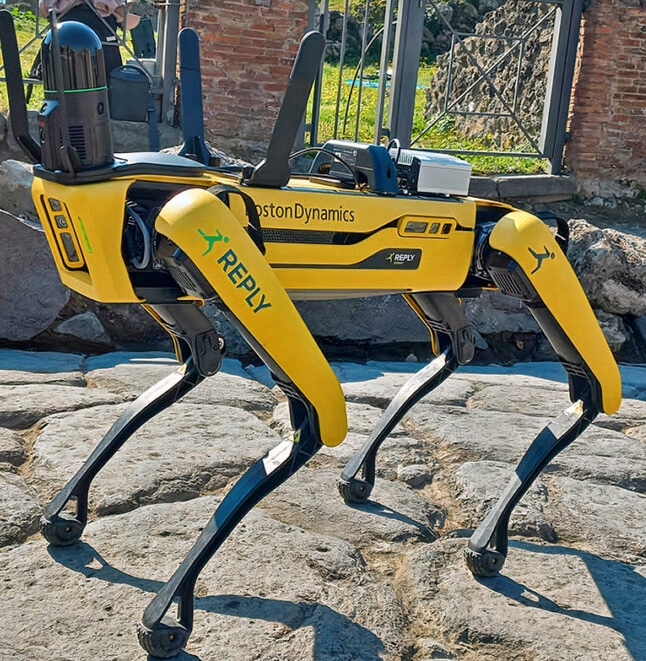
\includegraphics[width=2.5cm]{data/spot.jpg}
            };
            \node[inner sep=0pt, draw=black, label=below:\tiny{Sophia}] at (2.7, 1.9) {
                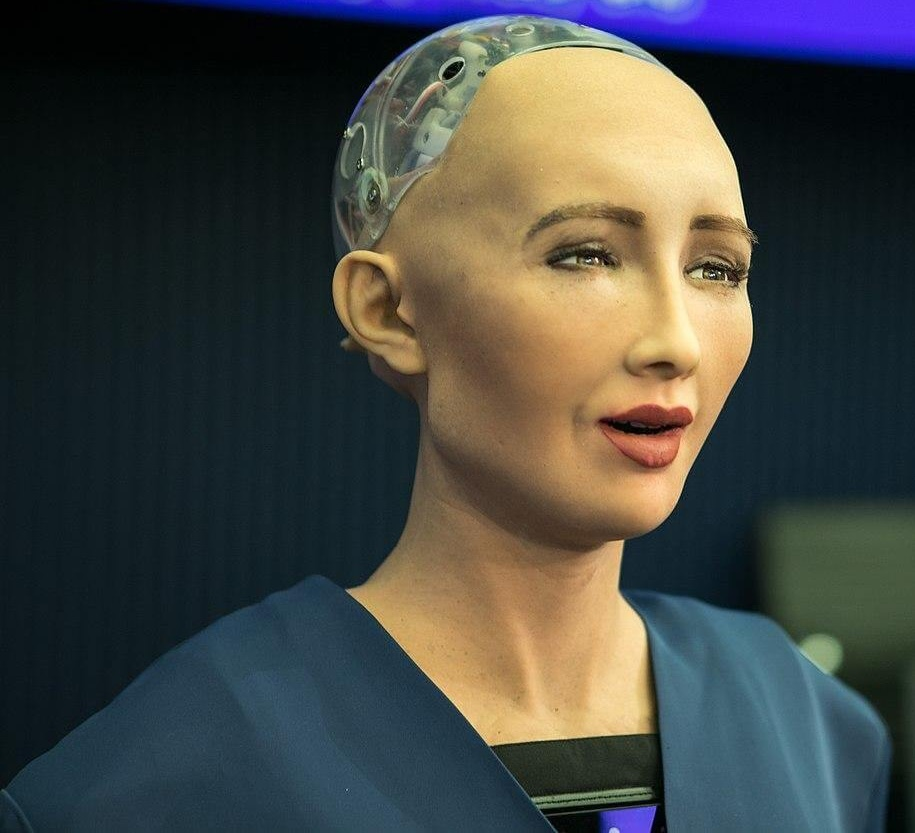
\includegraphics[width=2.5cm]{data/sophia.jpg}
            };
            \node[inner sep=0pt, draw=black, label=below:\tiny{AlphaFold}] at (1, -1.8) {
                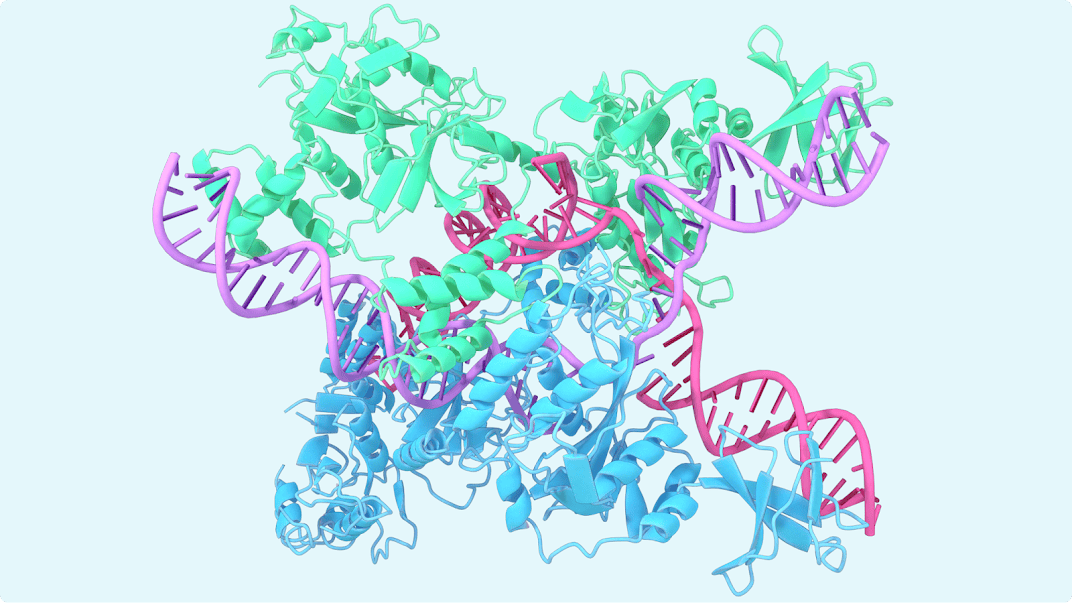
\includegraphics[width=3cm]{data/alphafold.png}
            };
            \node[inner sep=0pt, draw=black, label=below:\tiny{AlphaZero}] at (4.5, -1.1) {
                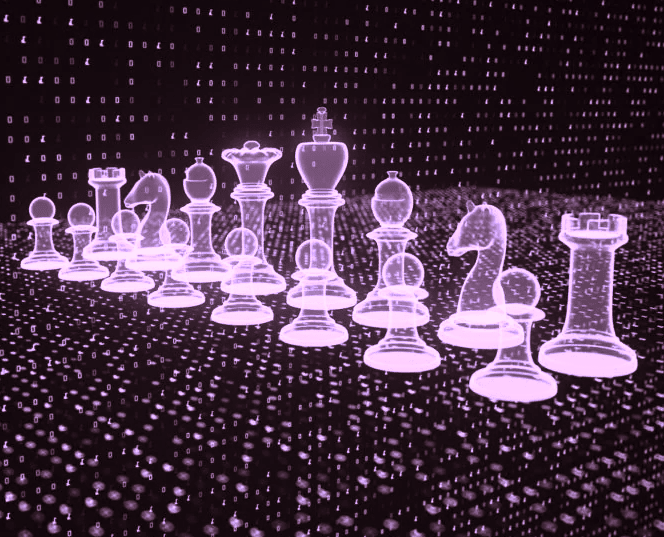
\includegraphics[width=2.7cm]{data/chess.png}
            };
        }

        \only<2>{
            \node[circle, fill=uioblue!80, minimum size=6cm, anchor=north] (ai) at (-4, 3.25) {};
            \node[white, anchor=north, align=center, font=\small\bfseries\linespread{0.9}\selectfont] at ($ (ai.north) - (0, 0.1) $) {Artificial\\intelligence};
            \node[align=flush left, anchor=north west, text width=7.2cm, font=\small\linespread{0.95}\selectfont] (def1) at (-0.5, 3.25) {
                \textbf{Artificial intelligence}\\
                The field of study producing technology that solves tasks requiring some form of intelligence
            };
            \node[circle, fill=uioblue!50!uiored!80, anchor=south, minimum size=4.1cm] (ml) at ($ (ai.south) + (0, 0.05) $) {};
            \node[white, anchor=north, align=center, font=\small\bfseries\linespread{0.9}\selectfont] at ($ (ml.north) - (0, 0.1) $) {Machine\\learning};
            \node[align=center, font=\small\linespread{0.9}\selectfont, text=white] at ($ (ai.north) + (1.3, -1.5) $) {Rule-based\\systems};
            \node[align=flush left, anchor=north west, text width=7.2cm, font=\small\linespread{0.95}\selectfont] (def2) at (def1.south west) {
                \textbf{Machine learning}\\
                A set of techniques to solve problems by allowing machines to find patterns in training data
            };
            \node[circle, fill=uiored!80, anchor=south, minimum size=3cm] (dl) at ($ (ml.south) + (0, 0.06) $) {};
            \node[white, anchor=north, align=center, font=\small\bfseries\linespread{0.9}\selectfont] at ($ (dl.north) - (0, 0.1) $) {Deep\\learning};
            \node[align=flush left, anchor=north west, text width=7.2cm, font=\small\linespread{0.95}\selectfont] (def3) at (def2.south west) {
                \textbf{Deep learning}\\
                    Machine learning approaches that rely on artificial neural networks
                };

        }
    \end{tikzpicture}
\end{frame}

\newcommand{\brainsize}[1]{
    \begin{tikzpicture}
        \begin{axis}[
            width=8cm,
            height=3.8cm,
            xlabel=\footnotesize{Age},
            ylabel=\footnotesize{Brain size},
            xmajorticks=false,
            ymajorticks=false,
            axis lines=left,
            xmin=2,
            xmax=13,
            ymin=935,
            ymax=1600
        ]
            \addplot[
                only marks,
                uioblue,
                opacity=0.5
            ] table [
                col sep=comma,
                x=x,
                y=y
            ] {data/brainsize.csv};

            \ifnum#1=1
                \addplot[
                    samples=100,
                    domain=2:15,
                    very thick,
                    uioblue
                ] {
                    1064.062904437416+x*36.95459273
                };
            \fi
            \ifnum#1=2
                \addplot[
                    samples=100,
                    domain=2:15,
                    very thick,
                    uioblue
                ] {
                    400+1100*(1-e^(-x/3))
                };
            \fi
        \end{axis}
    \end{tikzpicture}
}

\begin{frame}{Why do we use artificial neural networks?}
    \begin{tikzpicture}
        \node[] at (-7, -3.25) {};
        \node[] at (7, 3.25) {};

        \visible<1-3>{
            \node[anchor=east] (input) at (-3, 1.25) {$\text{input}$};
            \node[anchor=west] (output) at (3, 1.25) {$\text{output}$};
        }
        \visible<2>{
            \node[] at (-0.25, -1.85) {
                \brainsize{0}
            };
        }
        \visible<3>{
            \node[] at (-0.25, -1.85) {
                \brainsize{2}
            };
        }
        \visible<4>{
            \node[anchor=east, inner sep=0pt, draw=black] (input) at (-3, 1.25) {
                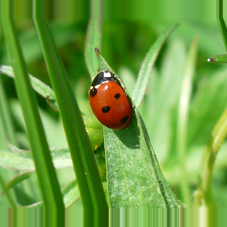
\includegraphics[width=2.5cm]{data/ladybug.png}
            };
            \node[anchor=west] (output) at (3, 1.25) {$\text{ladybug}$};
        }
        \visible<5>{
            \node[anchor=east, inner sep=0pt] (input1) at (-4, 2.75) {
                {\Huge{\emoji{spiral-notepad}}}
            };
            \node[anchor=east, inner sep=0pt, draw=black] (input2) at (-4, 1.25) {
                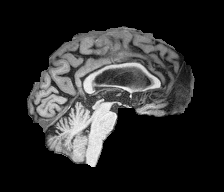
\includegraphics[width=1.5cm]{data/mri_sagittal.png}
            };
            \node[anchor=east, inner sep=0pt] (input3) at (-4, -0.25) {
                {\Huge{\emoji{microscope}}}
            };
            \node[anchor=west, align=left] (output) at (3, 1.25) {
                Clinical\\
                prediction
            };
        }

        \node[fill=gray!80, minimum width=4cm, minimum height=2.9cm, rounded corners=0.1cm, text=white, draw=black, font=\systemfont, anchor=south, text depth=2.4cm] (model) at (0, 0) {
            Artificial neural network
        };
        \only<1-4>{
            \draw[-stealth] (input.east) -- ($ (model.south west) + (0, 1.25) $);
        }
        \draw[-stealth] ($ (model.south east) + (0, 1.25) $) -- (output);
        \neuron{n00}{($ (model.south) + (0, 1.25) + (-2*\hsep, -2*\vsep) $)}
        \neuron{n01}{($ (n00) + (0, \vsep) $)}
        \neuron{n02}{($ (n00) + (0, 2*\vsep) $)}
        \neuron{n03}{($ (n00) + (0, 3*\vsep) $)}
        \neuron{n04}{($ (n00) + (0, 4*\vsep) $)}

        \neuron{n10}{($ (n00) + (\hsep, 0.5*\vsep) $)}
        \neuron{n11}{($ (n00) + (\hsep, 1.5*\vsep) $)}
        \neuron{n12}{($ (n00) + (\hsep, 2.5*\vsep) $)}
        \neuron{n13}{($ (n00) + (\hsep, 3.5*\vsep) $)}

        \neuron{n20}{($ (n00) + (2*\hsep, \vsep) $)}
        \neuron{n21}{($ (n00) + (2*\hsep, 2*\vsep) $)}
        \neuron{n22}{($ (n00) + (2*\hsep, 3*\vsep) $)}

        \neuron{n30}{($ (n00) + (3*\hsep, 1.5*\vsep) $)}
        \neuron{n31}{($ (n00) + (3*\hsep, 2.5*\vsep) $)}

        \neuron{n40}{($ (n00) + (4*\hsep, 2*\vsep) $)}

        \foreach \j in {0,...,4} {
            \draw[black, opacity=\edgeopacity] ($ (model.west) - (0, 0.2175) $) -- (n0\j);
        }

        \foreach \j in {0,...,4} {
            \foreach \k in {0,...,3} {
                \draw[black, opacity=\edgeopacity] (n0\j) -- (n1\k);
            }
        }
        \foreach \j in {0,...,3} {
            \foreach \k in {0,...,2} {
                \draw[black, opacity=\edgeopacity] (n1\j) -- (n2\k);
            }
        }
        \foreach \j in {0,...,2} {
            \foreach \k in {0,...,1} {
                \draw[black, opacity=\edgeopacity] (n2\j) -- (n3\k);
            }
        }
        \draw[black, opacity=\edgeopacity] (n30) -- (n40);
        \draw[black, opacity=\edgeopacity] (n31) -- (n40);
        \draw[black, opacity=\edgeopacity] (n40) -- ($ (model.south east) + (0, 1.25) $);

        \only<1>{
            \node[circle, draw=black, fill=uiogreen, minimum size=0.5cm] (neuron) at ($ (model.south) - (0, 1.5) $) {};

            \node[anchor=east, font=\scriptsize] (x1) at ($ (neuron) - (0.75, -0.5) $) {$\text{input}_1$};
            \node[anchor=east, font=\scriptsize] (x2) at ($ (neuron) - (0.75, 0) $) {$\text{input}_2$};
            \node[anchor=east, font=\scriptsize] (x3) at ($ (neuron) - (0.75, 0.5) $) {$\text{input}_3$};

            \node[anchor=west, font=\scriptsize] (y) at ($ (neuron) + (0.75, 0) $) {$\text{output}$};

            \draw[-stealth] (x1) -- (neuron);
            \draw[-stealth] (x2) -- (neuron);
            \draw[-stealth] (x3) -- (neuron);
            \draw[-stealth] (neuron) -- (y);

            \node[font=\small] at ($ (neuron) + (0, 1) $) {
                Artificial neuron
            };
        }

        \only<5>{
            \draw[-stealth] (input1) -- ($ (model.south west) + (0, 1.25) $);
            \draw[-stealth] (input2) -- ($ (model.south west) + (0, 1.25) $);
            \draw[-stealth] (input3) -- ($ (model.south west) + (0, 1.25) $);
        }
    \end{tikzpicture}
\end{frame}
	\section{Integrating multimodal health data for clinical predictions}

\begin{frame}{Late fusion: independent insights, combined decisions}
    \begin{tikzpicture}
        \node[draw=black] at (-7, -3.25) {};
        \node[draw=black] at (7, 3.25) {};

        \only<1-2>{
            \node[anchor=east, inner sep=0pt] (input2) at (-4, 2) {
                {\Huge{\emoji{spiral-notepad}}}
            };
            \node[anchor=east, inner sep=0pt, draw=black] (input) at (-4, -0.25) {
                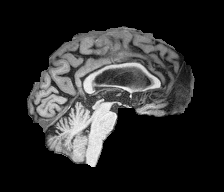
\includegraphics[width=1.5cm]{data/mri_sagittal.png}
            };
            \node[anchor=east, inner sep=0pt] (input3) at (-4, -2.5) {
                {\Huge{\emoji{microscope}}}
            };
        }
        \only<2>{
            \node[] (ehr) at (-1, 2.25) {
                \nn{EHR-specific ANN}{ehrnn}
            };
            \node[anchor=west, font=\small] (output1) at (2, 1.99) {EHR-index};
            \draw[-stealth] (input2) -- ($ (ehr.west) - (-0.12, 0.26) $);
            \draw[-stealth] ($ (ehr.east) - (0.25, 0.26) $) -- (output1);
            \node[] (mri) at (-1, 0) {
                \nn{MRI-specific ANN}{mrinn}
            };
            \node[anchor=west, font=\small] (output2) at (2, -0.26) {MRI-index};
            \draw[-stealth] (input) -- ($ (mri.west) - (-0.12, 0.26) $);
            \draw[-stealth] ($ (mri.east) - (0.25, 0.26) $) -- (output2);
            \node[] (bio) at (-1, -2.25) {
                \nn{Bio-specific ANN}{bionn}
            };
            \node[anchor=west, font=\small] (output3) at (2, -2.51) {Bio-index};
            \draw[-stealth] (input3) -- ($ (bio.west) - (-0.12, 0.26) $);
            \draw[-stealth] ($ (bio.east) - (0.25, 0.26) $) -- (output3);

            \node[anchor=east, font=\small, align=left] (output) at (7, -0.26) {Clinical\\prediction};
            \draw[-stealth] (output1.east) -- (output);
            \draw[-stealth] (output2.east) -- (output);
            \draw[-stealth] (output3.east) -- (output);
        }
        \only<3-5>{
            \node[anchor=south, font=\tiny\linespread{0.95}\selectfont, text width=11cm, align=flush center] at (0, -3.5) {
                Cordelli, E., et al., Machine learning predicts pulmonary Long Covid sequelae using clinical data, \textit{BMC Medical Informatics and Decision Making} (2024).
            };
        }
        \only<3>{
            % \node[inner sep=0pt, draw=black] at (0, 0) {
            %     
\includegraphics[width=10cm]{data/cordelli.png}
            % };
            \node[inner sep=0pt, draw=black] at (0, 2) {
                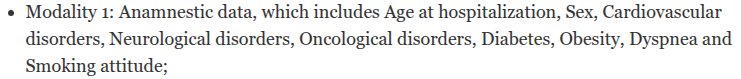
\includegraphics[width=9cm]{data/cordelli_modality_1.png}
            };
            \node[inner sep=0pt, draw=black] at (0, 0.1) {
                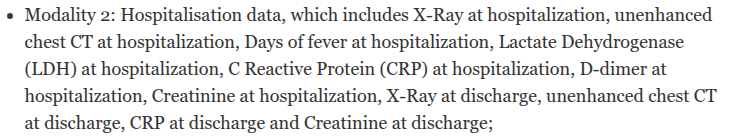
\includegraphics[width=9cm]{data/cordelli_modality_2.png}
            };
            \node[inner sep=0pt, draw=black] at (0, -1.8) {
                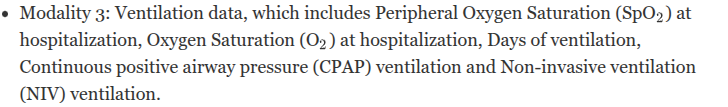
\includegraphics[width=9cm]{data/cordelli_modality_3.png}
            };
        }
        \only<4>{
            \node[inner sep=0pt, draw=black] at (0, 0.2) {
                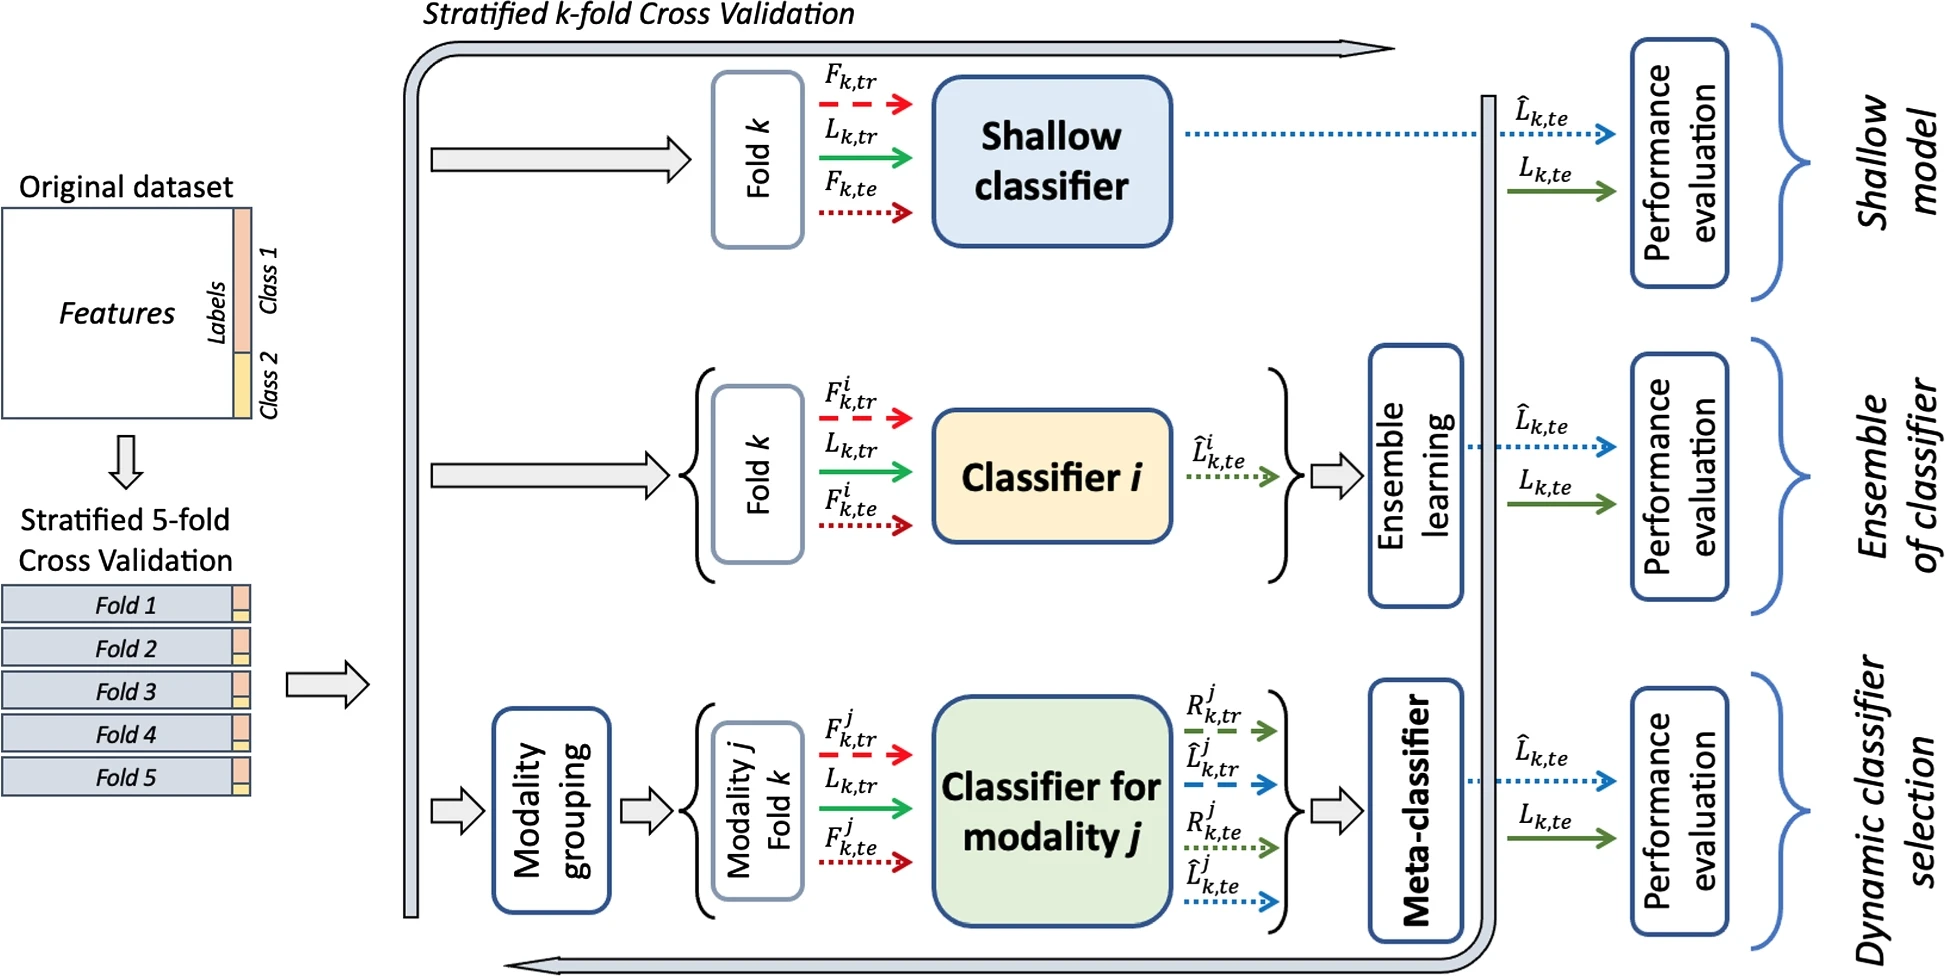
\includegraphics[width=11cm]{data/cordelli_model.png}
            };
        }
        \only<5>{
            \node[inner sep=0pt, draw=black] at (0, 0.2) {
                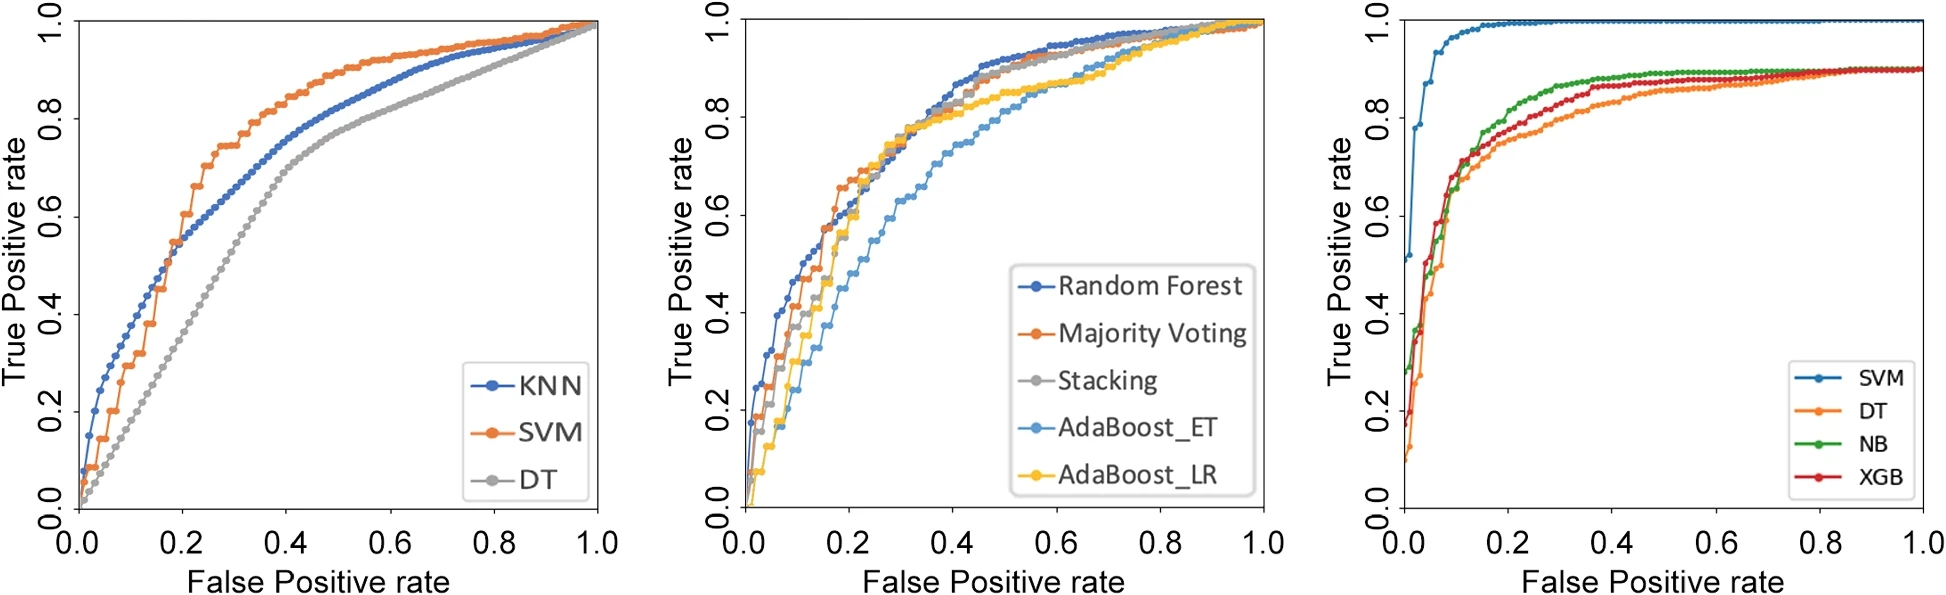
\includegraphics[width=12cm]{data/cordelli_results.png}
            };
        }
    \end{tikzpicture}
\end{frame}

\begin{frame}{Early fusion: blending information from the start}
    \begin{tikzpicture}
        \node[draw=black] at (-7, -3.25) {};
        \node[draw=black] at (7, 3.25) {};

        \only<1-3>{
            \node[fill=gray!80, minimum width=4cm, minimum height=2.9cm, rounded corners=0.1cm, text=white, draw=black, font=\systemfont, text depth=2.4cm, anchor=east] (ann) at (7, 0) {
                Modality-agnostic ANN
            };
            \only<1,3>{
                \neuron{n00}{($ (ann.south) + (0, 1.25) + (-2*\hsep, -2*\vsep) $)}
                \neuron{n01}{($ (n00) + (0, \vsep) $)}
                \neuron{n02}{($ (n00) + (0, 2*\vsep) $)}
                \neuron{n03}{($ (n00) + (0, 3*\vsep) $)}
                \neuron{n04}{($ (n00) + (0, 4*\vsep) $)}
            }
            \only<2>{
                \neuron[uioblue]{n00}{($ (ann.south) + (0, 1.25) + (-2*\hsep, -2*\vsep) $)}
                \neuron[uioblue]{n01}{($ (n00) + (0, \vsep) $)}
                \neuron[uiored]{n02}{($ (n00) + (0, 2*\vsep) $)}
                \neuron[uiored]{n03}{($ (n00) + (0, 3*\vsep) $)}
                \neuron[uioblue]{n04}{($ (n00) + (0, 4*\vsep) $)}
            }

            \only<1,3>{
                \neuron{n10}{($ (n00) + (\hsep, 0.5*\vsep) $)}
                \neuron{n11}{($ (n00) + (\hsep, 1.5*\vsep) $)}
                \neuron{n12}{($ (n00) + (\hsep, 2.5*\vsep) $)}
                \neuron{n13}{($ (n00) + (\hsep, 3.5*\vsep) $)}
            }
            \only<2>{
                \neuron[uiored]{n10}{($ (n00) + (\hsep, 0.5*\vsep) $)}
                \neuron[uiored]{n11}{($ (n00) + (\hsep, 1.5*\vsep) $)}
                \neuron[uioblue]{n12}{($ (n00) + (\hsep, 2.5*\vsep) $)}
                \neuron[uiored]{n13}{($ (n00) + (\hsep, 3.5*\vsep) $)}
            }

            \only<1,3>{
                \neuron{n20}{($ (n00) + (2*\hsep, \vsep) $)}
                \neuron{n21}{($ (n00) + (2*\hsep, 2*\vsep) $)}
                \neuron{n22}{($ (n00) + (2*\hsep, 3*\vsep) $)}
            }
            \only<2>{
                \neuron[uiored!60!uioblue]{n20}{($ (n00) + (2*\hsep, \vsep) $)}
                \neuron[uiored!75!uioblue]{n21}{($ (n00) + (2*\hsep, 2*\vsep) $)}
                \neuron[uioblue!75!uiored]{n22}{($ (n00) + (2*\hsep, 3*\vsep) $)}
            }

            \only<1>{
                \neuron{n30}{($ (n00) + (3*\hsep, 1.5*\vsep) $)}
                \neuron{n31}{($ (n00) + (3*\hsep, 2.5*\vsep) $)}
            }
            \only<2>{
                \neuron[uiored!50!uioblue]{n30}{($ (n00) + (3*\hsep, 1.5*\vsep) $)}
                \neuron[uiored!50!uioblue]{n31}{($ (n00) + (3*\hsep, 2.5*\vsep) $)}
            }
            \only<3>{
                \neuron{n30}{($ (n00) + (3*\hsep, 1.5*\vsep) $)}
                \neuron[yellow]{n31}{($ (n00) + (3*\hsep, 2.5*\vsep) $)}
            }

            \only<1,3>{
                \neuron{n40}{($ (n00) + (4*\hsep, 2*\vsep) $)}
            }
            \only<2>{
                \neuron[uiored!50!uioblue]{n40}{($ (n00) + (4*\hsep, 2*\vsep) $)}
            }

            \foreach \j in {0,...,4} {
                \draw[black, opacity=\edgeopacity] ($ (ann.west) - (0, 0.2175) $) -- (n0\j);
            }

            \foreach \j in {0,...,4} {
                \foreach \k in {0,...,3} {
                    \draw[black, opacity=\edgeopacity] (n0\j) -- (n1\k);
                }
            }
            \foreach \j in {0,...,3} {
                \foreach \k in {0,...,2} {
                    \draw[black, opacity=\edgeopacity] (n1\j) -- (n2\k);
                }
            }
            \foreach \j in {0,...,2} {
                \foreach \k in {0,...,1} {
                    \draw[black, opacity=\edgeopacity] (n2\j) -- (n3\k);
                }
            }
            \draw[black, opacity=\edgeopacity] (n30) -- (n40);
            \draw[black, opacity=\edgeopacity] (n31) -- (n40);
            \draw[black, opacity=\edgeopacity] (n40) -- ($ (ann.south east) + (0, 1.25) $);

            \node[anchor=east, inner sep=0pt] (text) at ($ (ann.south) + (0, 1.25) + (-10, 1.5) $) {
                {\Huge{\emoji{spiral-notepad}}}
            };
            \node[draw=black, align=center, rounded corners=0.1cm, anchor=west, font=\small] (texttokenizer) at ($ (text.east) + (1, 0) $) {Text\\tokenizer};
            \only<1-2>{
                \node[font=\scriptsize, inner sep=1pt, draw=black, anchor=west, text depth=0] (texttoken1) at ($ (texttokenizer.east) + (1, 0) $) {The};
                \node[font=\scriptsize, inner sep=1pt, draw=black, anchor=west, text depth=0] (texttoken2) at ($ (texttoken1.east) + (0.1, 0) $) {patient};
                \node[font=\scriptsize, inner sep=1pt, draw=black, anchor=west, text depth=0] (texttoken3) at ($ (texttoken2.east) + (0.1, 0) $) {has};
            }
            \only<3>{
                \node[font=\scriptsize, inner sep=1pt, draw=black, text depth=0] (texttoken2) at ($ (texttoken1.west)!0.5!(texttoken3.east) $) {Spiderman};
            }
            \draw[dashed, uioblue, thick] ($ (texttoken1.north west) + (-0.1, 0.1) $) -- ($ (texttoken3.north east) + (0.1, 0.1) $) -- ($ (texttoken3.south east) + (0.1, -0.1) $) -- ($ (texttoken1.south west) + (-0.1, -0.1) $) -- cycle;
            \node[anchor=south, text=uioblue, font=\scriptsize, inner sep=0pt] at ($ (texttoken2.north) + (0, 0.2) $) {Text tokens};
            \draw[-stealth] (text) -- (texttokenizer);
            \draw[-stealth] (texttokenizer) -- ($ (texttoken1.west) - (0.1, 0) $);
            \draw[-stealth] ($ (texttoken3.east) + (0.1, 0) $) -| ($ (ann.south west) + (-1, 1.25) $) --  ($ (ann.south west) + (0, 1.25) $);

            \node[anchor=east, inner sep=0pt, draw=black] (mri) at ($ (ann.south) + (0, 1.25) + (-10, -1.5) $) {
                \only<1-2>{%
                    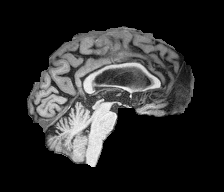
\includegraphics[width=1.5cm]{data/mri_sagittal.png}
                }%
                \only<3>{%
                    
\includegraphics[width=1.5cm]{data/spiderman.png}
                }%
            };
            \node[draw=black, align=center, rounded corners=0.1cm, anchor=west, font=\small] (mritokenizer) at ($ (mri.east) + (1, 0) $) {Image\\tokenizer};
            \node[anchor=west, inner sep=0pt] (mritoken1) at ($ (mritokenizer.east) + (1, 0) $) {
                \only<1-2>{%
                    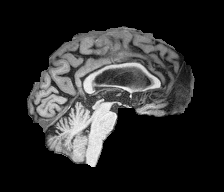
\includegraphics[
                        width=0.66cm,
                        trim={0cm 3.8cm 3.8cm 0cm},
                        clip
                    ]{data/mri_sagittal.png}
                }%
                \only<3>{%
                    
\includegraphics[
                        width=0.66cm,
                        trim={0cm 8cm 8cm 0cm},
                        clip
                    ]{data/spiderman.png}
                }%
            };
            \node[anchor=west, inner sep=0pt] (mritoken2) at ($ (mritoken1.east) + (0.1, 0) $) {
                \only<1-2>{%
                    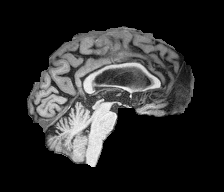
\includegraphics[
                        width=0.66cm,
                        trim={3.8cm 3.8cm 0cm 0cm},
                        clip
                    ]{data/mri_sagittal.png}
                }%
                \only<3>{%
                    
\includegraphics[
                        width=0.66cm,
                        trim={8cm 8cm 0cm 0cm},
                        clip
                    ]{data/spiderman.png}
                }%
            };
            \node[anchor=west, inner sep=0pt] (mritoken3) at ($ (mritoken2.east) + (0.1, 0) $) {
                \only<1-2>{%
                    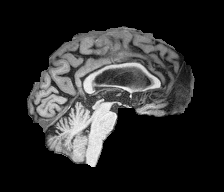
\includegraphics[
                        width=0.66cm,
                        trim={0cm 0cm 3.8cm 3.8cm},
                        clip
                    ]{data/mri_sagittal.png}
                }%
                \only<3>{%
                    
\includegraphics[
                        width=0.66cm,
                        trim={0cm 0cm 8cm 8cm},
                        clip
                    ]{data/spiderman.png}
                }%
            };
            \draw[dashed, uiored, thick] ($ (mritoken1.north west) + (-0.1, 0.1) $) -- ($ (mritoken3.north east) + (0.1, 0.1) $) -- ($ (mritoken3.south east) + (0.1, -0.1) $) -- ($ (mritoken1.south west) + (-0.1, -0.1) $) -- cycle;
            \node[anchor=north, text=uiored, font=\scriptsize, inner sep=0pt] at ($ (mritoken2.south) - (0, 0.2) $) {Image tokens};

            \draw[-stealth] (mri) -- (mritokenizer);
            \draw[-stealth] (mritokenizer) -- ($ (mritoken1.west) - (0.1, 0) $);
            \draw[-stealth] ($ (mritoken3.east) + (0.1, 0) $) -| ($ (ann.south west) + (-1, 1.25) $) --  ($ (ann.south west) + (0, 1.25) $);
        }
        \only<4>{
            \node[inner sep=0pt, draw=black] at (0, 0) {
                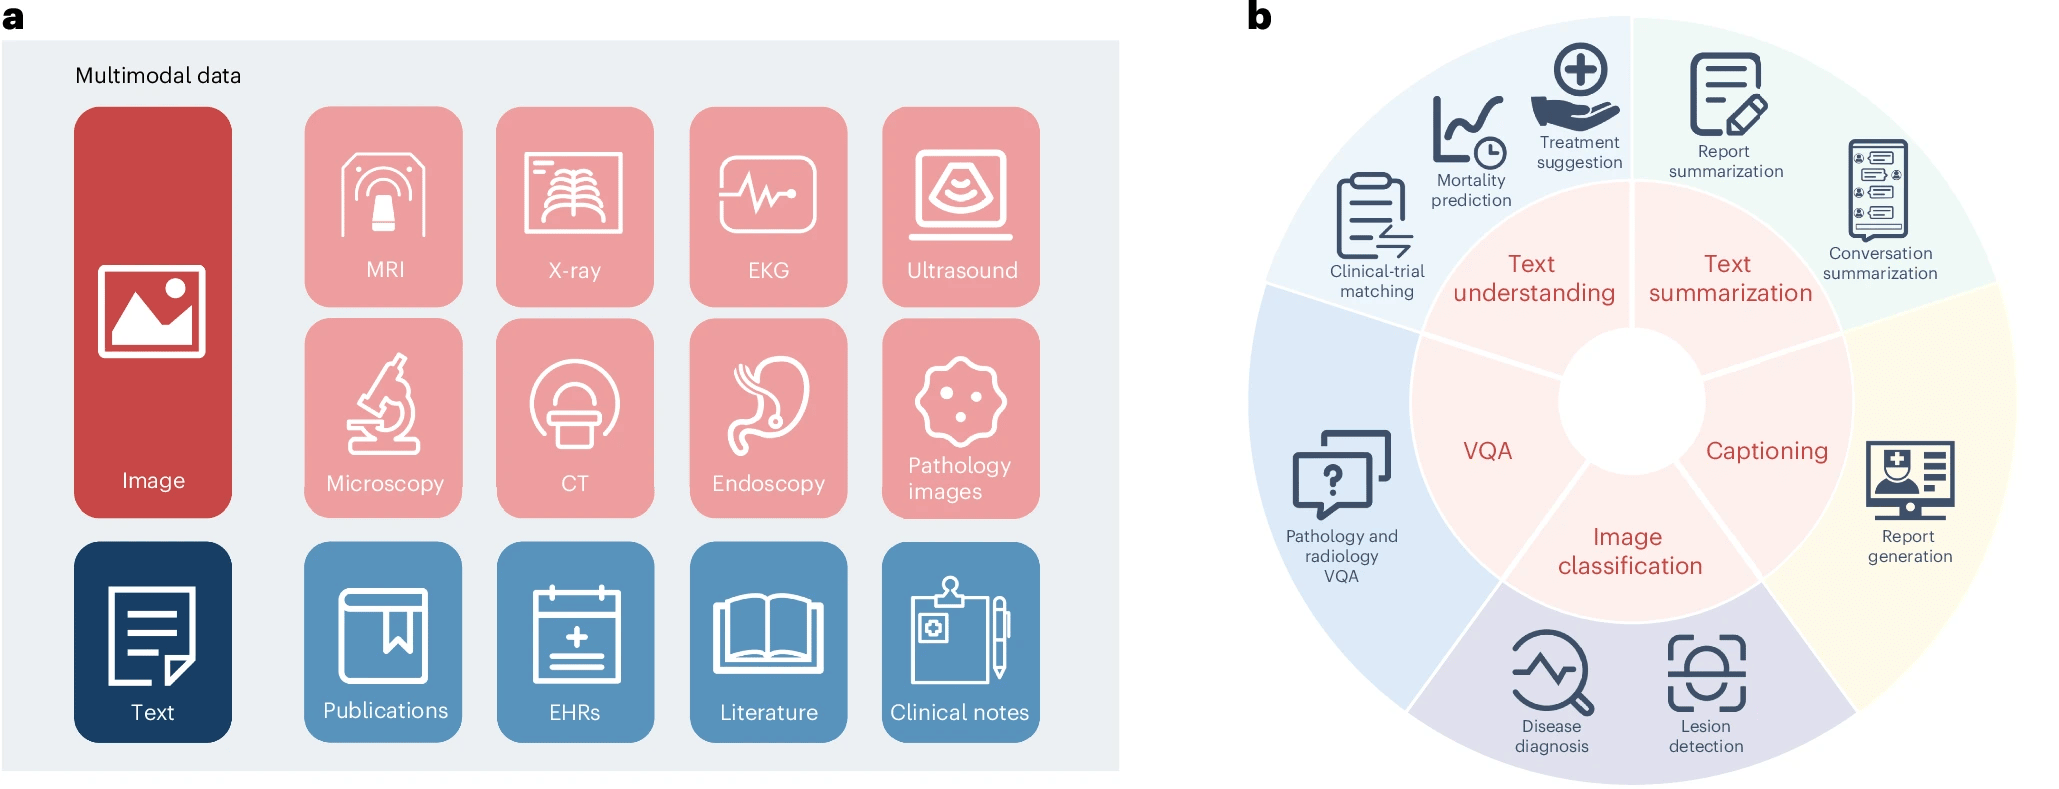
\includegraphics[width=12cm]{data/sun_modalities.png}
            };
        }
        \only<5>{
            \node[inner sep=0pt, draw=black] at (0, 0) {
                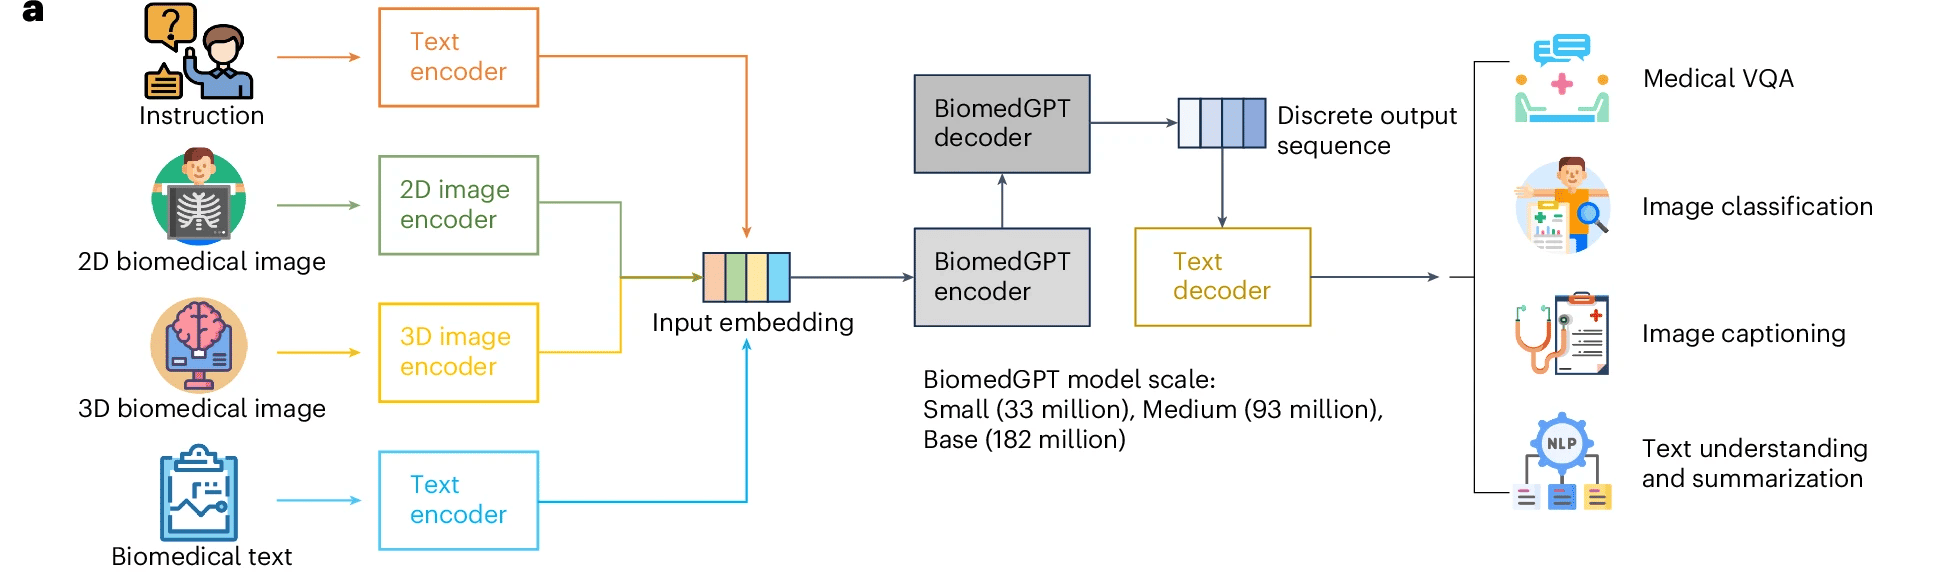
\includegraphics[width=12.5cm]{data/sun_model.png}
            };
        }
        \only<6>{
            \node[inner sep=0pt, draw=black] at (0, 0) {
                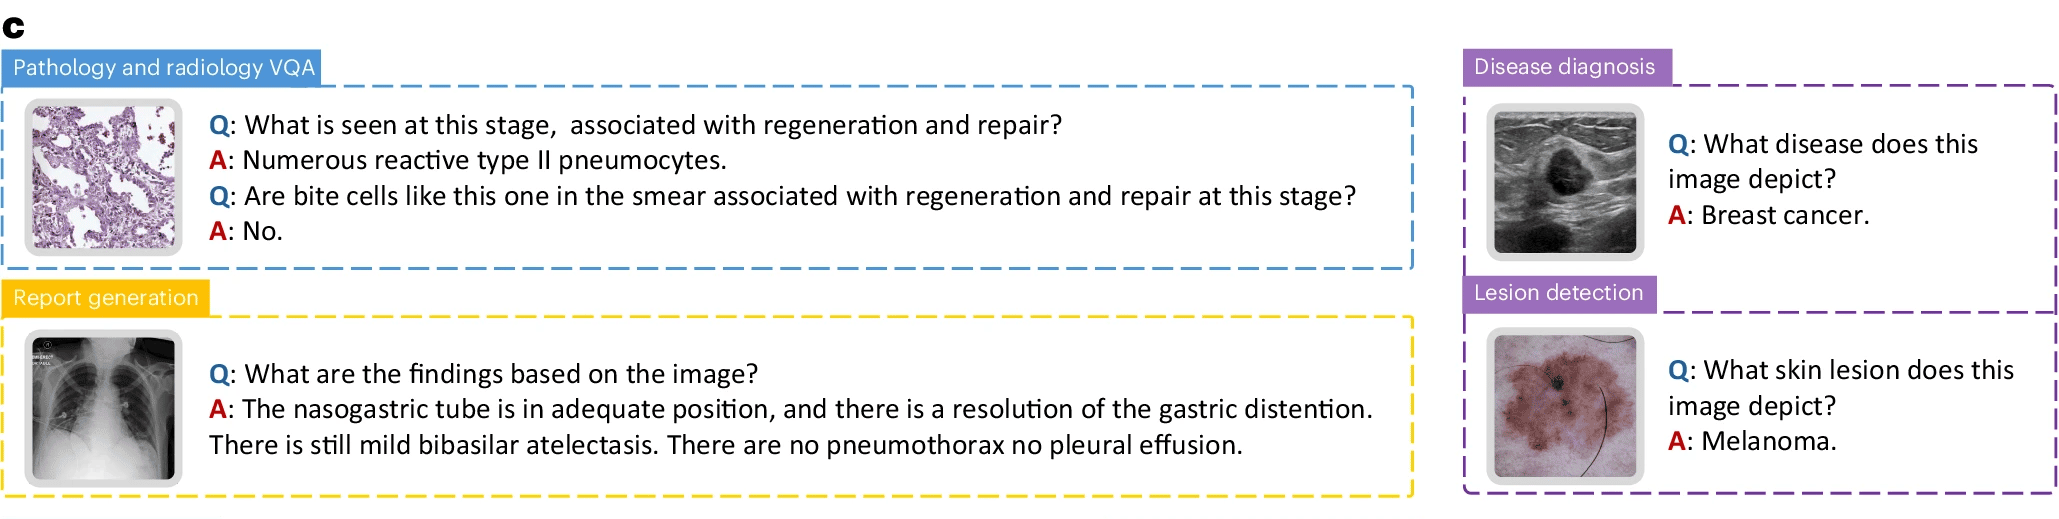
\includegraphics[width=11cm]{data/sun_questions.png}
            };
        }
        \only<7>{
            \node[inner sep=0pt, draw=black] at (0, 0) {
                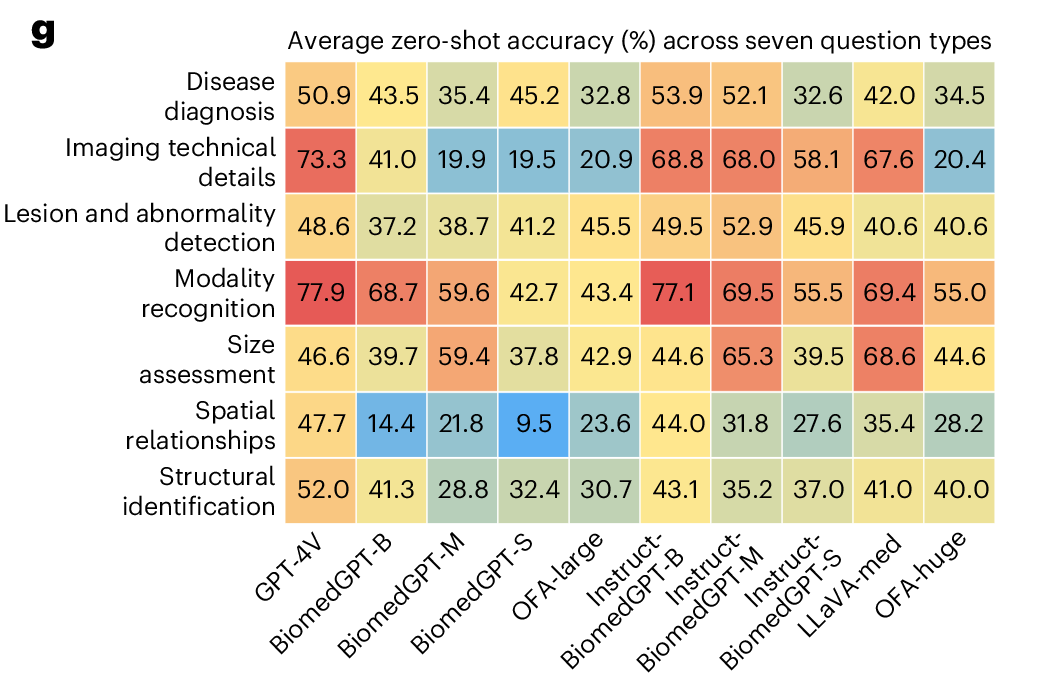
\includegraphics[width=7cm]{data/sun_tasks.png}
            };
        }

        \only<4-7>{
            \node[anchor=south, font=\tiny\linespread{0.95}\selectfont, text width=11cm, align=flush center] at (0, -3.5) {
                Zhang, K., et al., A generalist vision–language foundation model for diverse biomedical tasks, \textit{Nature Medicine} (2024).
            };
        }

    \end{tikzpicture}
\end{frame}

\begin{frame}{Intermediate fusion: integrating insights along the way}
    \begin{tikzpicture}
        \node[draw=black] at (-7, -3.25) {};
        \node[draw=black] at (7, 3.25) {};

        \only<1>{
            \node[fill=gray!80, minimum width=6cm, minimum height=6.5cm, rounded corners=0.1cm, text=white, draw=black, font=\systemfont, text depth=6cm] (multi) at (-0.6, 0.2) {
                Multimodal ANN
            };

            \node[] (ehr) at ($ (multi) - (1.85, -1.8) $) {
                \encoder{EHR encoder}{ehrenc}
            };
            \node[] (mri) at ($ (multi) - (1.85, 0.2) $) {
                \encoder{MRI encoder}{mrienc}
            };
            \node[] (bio) at ($ (multi) - (1.85, 2.2) $) {
                \encoder{Bio encoder}{bioenc}
            };


            \node[anchor=east, inner sep=0pt] (input2) at ($ (ehr.west) - (1, 0.2) $) {
                {\Huge{\emoji{spiral-notepad}}}
            };
            \draw[-stealth] (input2) -- ($ (ehr.west) - (-0.1, 0.2) $);
            \node[anchor=east, inner sep=0pt, draw=black] (input) at ($ (mri.west) - (1, 0.2) $) {
                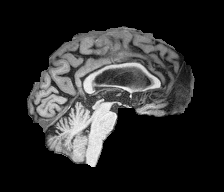
\includegraphics[width=1.5cm]{data/mri_sagittal.png}
            };
            \draw[-stealth] (input) -- ($ (mri.west) - (-0.1, 0.2) $);
            \node[anchor=east, inner sep=0pt] (input3) at ($ (bio.west) - (1, 0.2) $) {
                {\Huge{\emoji{microscope}}}
            };
            \draw[-stealth] (input3) -- ($ (bio.west) - (-0.1, 0.2) $);

            \neuron{n00}{($ (multi.south) + (0, 1.85) + (-0.5*\hsep, -2*\vsep) $)}
            \neuron{n01}{($ (n00) + (0, 2*\vsep) $)}
            \neuron{n02}{($ (n00) + (0, 4*\vsep) $)}
            \neuron{n03}{($ (n00) + (0, 6*\vsep) $)}
            \neuron{n04}{($ (n00) + (0, 8*\vsep) $)}
            \neuron{n10}{($ (n00) + (\hsep, 1*\vsep) $)}
            \neuron{n11}{($ (n00) + (\hsep, 3*\vsep) $)}
            \neuron{n12}{($ (n00) + (\hsep, 5*\vsep) $)}
            \neuron{n13}{($ (n00) + (\hsep, 7*\vsep) $)}

            \neuron{n20}{($ (n00) + (2*\hsep, 2*\vsep) $)}
            \neuron{n21}{($ (n00) + (2*\hsep, 4*\vsep) $)}
            \neuron{n22}{($ (n00) + (2*\hsep, 6*\vsep) $)}

            \neuron{n30}{($ (n00) + (3*\hsep, 3*\vsep) $)}
            \neuron{n31}{($ (n00) + (3*\hsep, 5*\vsep) $)}

            \neuron{n40}{($ (n00) + (4*\hsep, 4*\vsep) $)}

            \foreach \j in {0,...,4} {
                \draw[black, opacity=\edgeopacity] ($ (ehr.east) - (0.77, -0.04) $) -- (n0\j);
                \draw[black, opacity=\edgeopacity] ($ (ehr.east) - (0.77, 0.46) $) -- (n0\j);
                \draw[black, opacity=\edgeopacity] ($ (mri.east) - (0.77, -0.04) $) -- (n0\j);
                \draw[black, opacity=\edgeopacity] ($ (mri.east) - (0.77, 0.46) $) -- (n0\j);
                \draw[black, opacity=\edgeopacity] ($ (bio.east) - (0.77, -0.04) $) -- (n0\j);
                \draw[black, opacity=\edgeopacity] ($ (bio.east) - (0.77, 0.46) $) -- (n0\j);
                \foreach \k in {0,...,3} {
                    \draw[black, opacity=\edgeopacity] (n0\j) -- (n1\k);
                }
            }
            \foreach \j in {0,...,3} {
                \foreach \k in {0,...,2} {
                    \draw[black, opacity=\edgeopacity] (n1\j) -- (n2\k);
                }
            }
            \foreach \j in {0,...,2} {
                \foreach \k in {0,...,1} {
                    \draw[black, opacity=\edgeopacity] (n2\j) -- (n3\k);
                }
            }
            \draw[black, opacity=\edgeopacity] (n30) -- (n40);
            \draw[black, opacity=\edgeopacity] (n31) -- (n40);
            \draw[black, opacity=\edgeopacity] (n40) -- ($ (multi.south east) + (0, 2.85) $);

            \node[anchor=west, font=\small, align=left] (output) at ($ (multi.south east) + (1, 2.85) $) {Clinical\\prediction};
            \draw[-stealth] ($ (multi.south east) + (0, 2.85) $) -- (output);
        }
        \only<2>{
            \node[inner sep=0pt, draw=black, label=above:{Clinical notes}] at (0, -2.35) {
                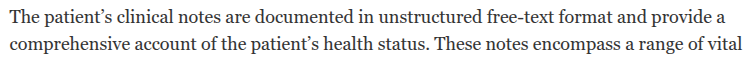
\includegraphics[width=7cm]{data/zhang_notes.png}
            };
            \node[inner sep=0pt, draw=black, label=above:{Multimodal MRI}] at (0, -0.3) {
                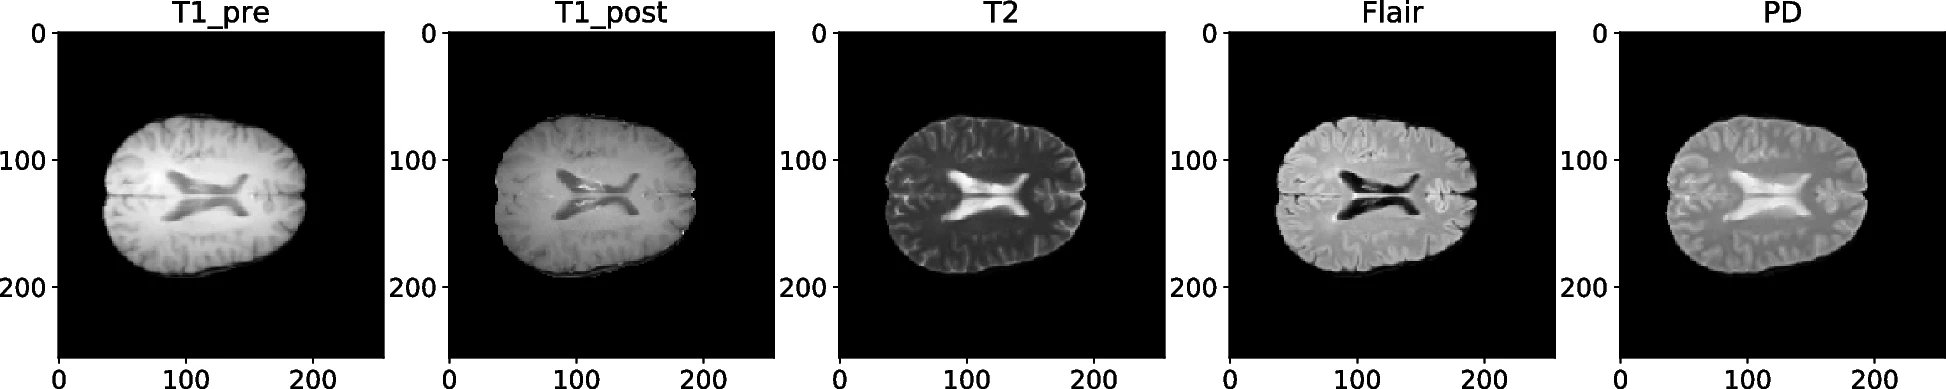
\includegraphics[width=9cm]{data/zhang_mri.png}
            };
            \node[inner sep=0pt, draw=black, label=above:{Structured EHR}] at (0, 2.25) {
                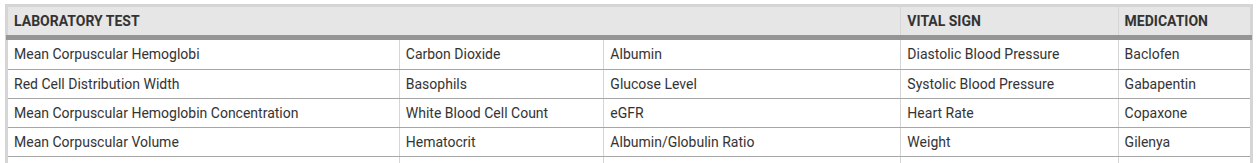
\includegraphics[width=7cm]{data/zhang_ehr.png}
            };
        }
        \only<3>{
            \node[inner sep=0pt, draw=black] at (0, 0.2) {
                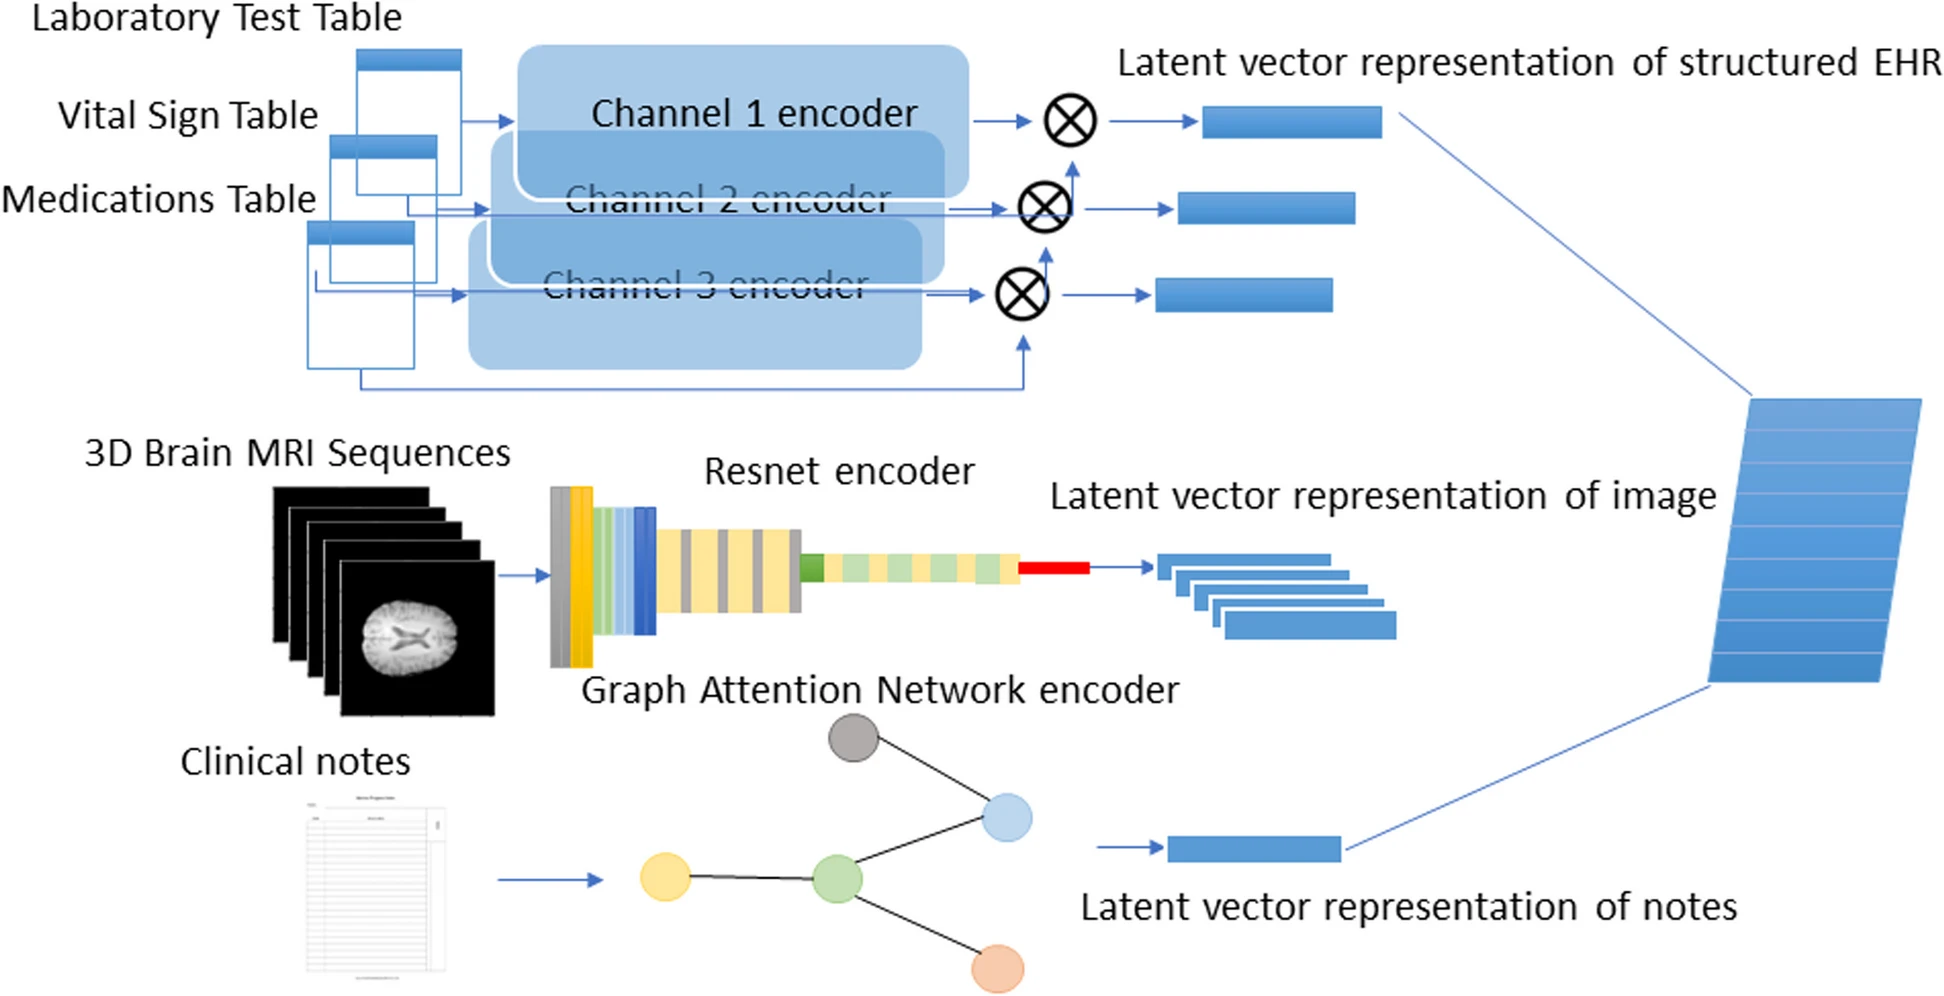
\includegraphics[width=10cm]{data/zhang_model.png}
            };
        }
        \only<4>{
            \node[inner sep=0pt, draw=black] at (0, 0) {
                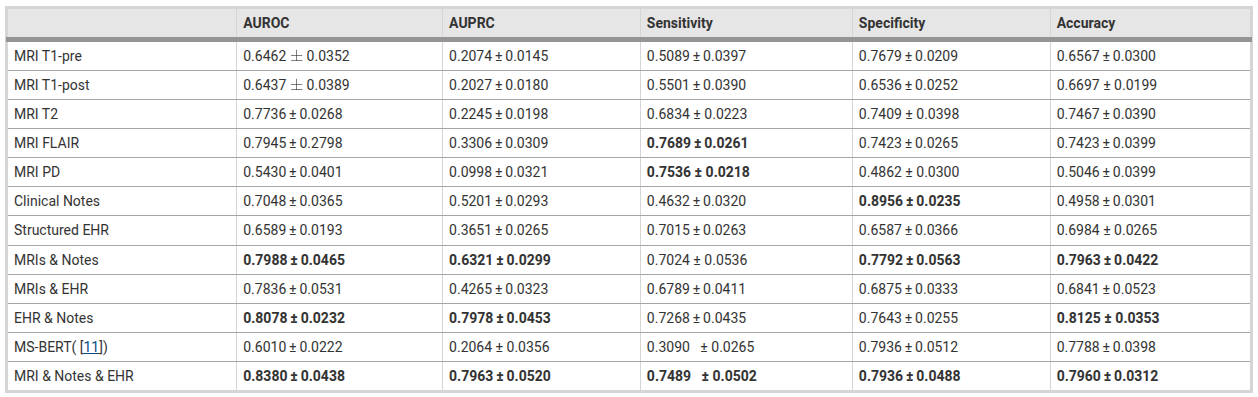
\includegraphics[width=13cm]{data/zhang_results.png}
            };
        }

        \only<2-4>{
            \node[anchor=south, font=\tiny\linespread{0.95}\selectfont, text width=11cm, align=flush center] at (0, -3.5) {
                Zhang, K., et al., Predicting multiple sclerosis severity with multimodal deep neural networks, \textit{BMC Medical Informatics and Decision Making} (2023).
            };
        }
    \end{tikzpicture}
\end{frame}
	\newcommand{\neuron}[3]{
    \node[circle, draw=black, fill=#2] (#1) at #3 {};
}

\begin{frame}{Explainable artificial intelligence}
    \begin{tikzpicture}
        \node[] at (-5.25, -3.5) {};
        \node[] at (5.25, 3.5) {};

        \node[
            draw=black,
            fill=cyan!15,
            minimum height=3cm,
            minimum width=4.3cm,
            label=above:\footnotesize{\textbf{Artificial neural network}}
        ] (model) at (0, 0) {};

        \def\hsep{0.7}
        \def\vsep{0.5}
        \def\edgecolor{gray}
        \def\edgeopacity{0.5}
        \def\neuroncolour{gray}

        \only<1>{
            \neuron{n00}{\neuroncolour}{($ (model) + (-2 * \hsep, -2 * \vsep) $)}
            \neuron{n01}{\neuroncolour}{($ (model) + (-2 * \hsep, -\vsep) $)}
            \neuron{n02}{\neuroncolour}{($ (model) + (-2 * \hsep, 0) $)}
            \neuron{n03}{\neuroncolour}{($ (model) + (-2 * \hsep, \vsep) $)}
            \neuron{n04}{\neuroncolour}{($ (model) + (-2 * \hsep, 2 * \vsep) $)}

            \neuron{n10}{\neuroncolour}{($ (model) + (-\hsep, -1.5 * \vsep) $)}
            \neuron{n11}{\neuroncolour}{($ (model) + (-\hsep, -0.5 * \vsep) $)}
            \neuron{n12}{\neuroncolour}{($ (model) + (-\hsep, 0.5 * \vsep) $)}
            \neuron{n13}{\neuroncolour}{($ (model) + (-\hsep, 1.5 * \vsep) $)}

            \neuron{n20}{\neuroncolour}{($ (model) + (0, -\vsep) $)}
            \neuron{n21}{\neuroncolour}{(model)}
            \neuron{n22}{\neuroncolour}{($ (model) + (0, \vsep) $)}

            \neuron{n30}{\neuroncolour}{($ (model) + (\hsep, -0.5 * \vsep) $)}
            \neuron{n31}{\neuroncolour}{($ (model) + (\hsep, 0.5 * \vsep) $)}

            \neuron{n40}{\neuroncolour}{($ (model) + (2 * \hsep, 0) $)}

            \draw[-stealth, \edgecolor, opacity=\edgeopacity] (model.west) -- (n00);
            \draw[-stealth, \edgecolor, opacity=\edgeopacity] (model.west) -- (n01);
            \draw[-stealth, \edgecolor, opacity=\edgeopacity] (model.west) -- (n02);
            \draw[-stealth, \edgecolor, opacity=\edgeopacity] (model.west) -- (n03);
            \draw[-stealth, \edgecolor, opacity=\edgeopacity] (model.west) -- (n04);

            \foreach \i in {0,...,4} {
                \foreach \j in {0,...,3} {
                    \draw[\edgecolor, opacity=\edgeopacity] (n0\i) -- (n1\j);
                }
            }
            \foreach \i in {0,...,3} {
                \foreach \j in {0,...,2} {
                    \draw[\edgecolor, opacity=\edgeopacity] (n1\i) -- (n2\j);
                }
            }
            \foreach \i in {0,...,2} {
                \foreach \j in {0,...,1} {
                    \draw[\edgecolor, opacity=\edgeopacity] (n2\i) -- (n3\j);
                }
            }
            \foreach \i in {0,...,1} {
                \draw[\edgecolor, opacity=\edgeopacity] (n3\i) -- (n40);
            }

            \draw[-stealth, \edgecolor, opacity=\edgeopacity] (n40) -- (model.east);
        }
        \only<2>{
            \neuron{n00}{black!25}{($ (model) + (-2 * \hsep, -2 * \vsep) $)}
            \neuron{n01}{black!90}{($ (model) + (-2 * \hsep, -\vsep) $)}
            \neuron{n02}{black!72}{($ (model) + (-2 * \hsep, 0) $)}
            \neuron{n03}{black!99}{($ (model) + (-2 * \hsep, \vsep) $)}
            \neuron{n04}{black!10}{($ (model) + (-2 * \hsep, 2 * \vsep) $)}

            \neuron{n10}{black!55}{($ (model) + (-\hsep, -1.5 * \vsep) $)}
            \neuron{n11}{black!92}{($ (model) + (-\hsep, -0.5 * \vsep) $)}
            \neuron{n12}{black!31}{($ (model) + (-\hsep, 0.5 * \vsep) $)}
            \neuron{n13}{black!7}{($ (model) + (-\hsep, 1.5 * \vsep) $)}

            \neuron{n20}{black!50}{($ (model) + (0, -\vsep) $)}
            \neuron{n21}{black!10}{(model)}
            \neuron{n22}{black!100}{($ (model) + (0, \vsep) $)}

            \neuron{n30}{black!75}{($ (model) + (\hsep, -0.5 * \vsep) $)}
            \neuron{n31}{black!65}{($ (model) + (\hsep, 0.5 * \vsep) $)}

            \neuron{n40}{black!95}{($ (model) + (2 * \hsep, 0) $)}

            \draw[-stealth, \edgecolor, opacity=\edgeopacity] (model.west) -- (n00);
            \draw[-stealth, \edgecolor, opacity=\edgeopacity] (model.west) -- (n01);
            \draw[-stealth, \edgecolor, opacity=\edgeopacity] (model.west) -- (n02);
            \draw[-stealth, \edgecolor, opacity=\edgeopacity] (model.west) -- (n03);
            \draw[-stealth, \edgecolor, opacity=\edgeopacity] (model.west) -- (n04);

            \foreach \i in {0,...,4} {
                \foreach \j in {0,...,3} {
                    \draw[\edgecolor, opacity=\edgeopacity] (n0\i) -- (n1\j);
                }
            }
            \foreach \i in {0,...,3} {
                \foreach \j in {0,...,2} {
                    \draw[\edgecolor, opacity=\edgeopacity] (n1\i) -- (n2\j);
                }
            }
            \foreach \i in {0,...,2} {
                \foreach \j in {0,...,1} {
                    \draw[\edgecolor, opacity=\edgeopacity] (n2\i) -- (n3\j);
                }
            }
            \foreach \i in {0,...,1} {
                \draw[\edgecolor, opacity=\edgeopacity] (n3\i) -- (n40);
            }

            \draw[-stealth, \edgecolor, opacity=\edgeopacity] (n40) -- (model.east);

            \node[anchor=east, draw=black, inner sep=0pt] (input) at ($ (model.west) + (-0.77, 0) $) {
                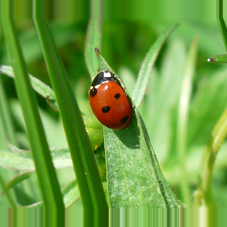
\includegraphics[width=2cm]{data/ladybug.png}
            };
            \cnnarrow{(input.east)}{(model.west)}{black}

            \node[anchor=west] (output) at ($ (model.east) + (0.77, 0) $) {
                Ladybug
            };
            \cnnarrow{(model.east)}{(output.west)}{black}

            \draw[-Latex, line width=3pt] ($ (model.south west) + (0.1, -0.4) $) -- ($ (model.south east) + (-0.1, -0.4) $);

            \node[] at (0, -2.3) {
                \textit{Forward pass}
            };
        }
        \only<3>{
            \neuron{n00}{red!25!black}{($ (model) + (-2 * \hsep, -2 * \vsep) $)}
            \neuron{n01}{red!90!black}{($ (model) + (-2 * \hsep, -\vsep) $)}
            \neuron{n02}{yellow!15!red}{($ (model) + (-2 * \hsep, 0) $)}
            \neuron{n03}{red!99!black}{($ (model) + (-2 * \hsep, \vsep) $)}
            \neuron{n04}{red!10!black}{($ (model) + (-2 * \hsep, 2 * \vsep) $)}

            \neuron{n10}{red!55!black}{($ (model) + (-\hsep, -1.5 * \vsep) $)}
            \neuron{n11}{yellow!20!red}{($ (model) + (-\hsep, -0.5 * \vsep) $)}
            \neuron{n12}{yellow!90!red}{($ (model) + (-\hsep, 0.5 * \vsep) $)}
            \neuron{n13}{red!7!black}{($ (model) + (-\hsep, 1.5 * \vsep) $)}

            \neuron{n20}{red!90!black}{($ (model) + (0, -\vsep) $)}
            \neuron{n21}{red!30!black}{(model)}
            \neuron{n22}{yellow!70!red}{($ (model) + (0, \vsep) $)}

            \neuron{n30}{yellow!40!red}{($ (model) + (\hsep, -0.5 * \vsep) $)}
            \neuron{n31}{red!65!black}{($ (model) + (\hsep, 0.5 * \vsep) $)}

            \neuron{n40}{red}{($ (model) + (2 * \hsep, 0) $)}

            \draw[stealth-, red, opacity=\edgeopacity] (model.west) -- (n00);
            \draw[stealth-, red, opacity=\edgeopacity] (model.west) -- (n01);
            \draw[stealth-, red, opacity=\edgeopacity] (model.west) -- (n02);
            \draw[stealth-, red, opacity=\edgeopacity] (model.west) -- (n03);
            \draw[stealth-, red, opacity=\edgeopacity] (model.west) -- (n04);

            \foreach \i in {0,...,4} {
                \foreach \j in {0,...,3} {
                    \draw[red, opacity=\edgeopacity] (n0\i) -- (n1\j);
                }
            }
            \foreach \i in {0,...,3} {
                \foreach \j in {0,...,2} {
                    \draw[red, opacity=\edgeopacity] (n1\i) -- (n2\j);
                }
            }
            \foreach \i in {0,...,2} {
                \foreach \j in {0,...,1} {
                    \draw[red, opacity=\edgeopacity] (n2\i) -- (n3\j);
                }
            }
            \foreach \i in {0,...,1} {
                \draw[red, opacity=\edgeopacity] (n3\i) -- (n40);
            }

            \draw[stealth-, red, opacity=\edgeopacity] (n40) -- (model.east);

            \node[anchor=east, draw=black, inner sep=0pt] (input) at ($ (model.west) + (-0.77, 0) $) {
                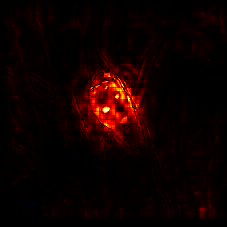
\includegraphics[width=2cm]{data/ladybug_explanation.png}
            };
            \lrparrow{(model.west)}{(input.east)}{red}

            \node[anchor=west, text=red] (output) at ($ (model.east) + (0.77, 0) $) {
                Ladybug
            };
            \lrparrow{(output.west)}{(model.east)}{red}

            \draw[Latex-, line width=3pt, red] ($ (model.south west) + (0.1, -0.4) $) -- ($ (model.south east) + (-0.1, -0.4) $);

            \node[text=red] at (0, -2.3) {
                \textit{Backward pass}
            };
        }
    \end{tikzpicture}
\end{frame}


\end{document}
